\documentclass[prb,12pt]{revtex4-2}
%fonts
% Palatino for main text and math
%\usepackage[osf,sc]{mathpazo}

% Helvetica for sans serif
% (scaled to match size of Palatino)
%\usepackage[scaled=0.90]{helvet}

% Bera Mono for monospaced
% (scaled to match size of Palatino)
%\usepackage[scaled=0.85]{beramono}
\usepackage{amsmath, amssymb,physics,amsfonts,amsthm}
\usepackage{enumitem}
\usepackage{cancel}
\usepackage{booktabs}
\usepackage{tikz}
\usepackage{hyperref}
\usepackage{enumitem}
\usepackage{transparent}
\usepackage{float}
\usepackage{multirow}
\newtheorem{Theorem}{Theorem}
\newtheorem{Proposition}{Theorem}
\newtheorem{Lemma}[Theorem]{Lemma}
\newtheorem{Corollary}[Theorem]{Corollary}
\newtheorem{Example}[Theorem]{Example}
\newtheorem{Remark}[Theorem]{Remark}
\theoremstyle{definition}
\newtheorem{Problem}{Aufgabe}
\theoremstyle{definition}
\newtheorem{Definition}[Theorem]{Definition}
\newenvironment{parts}{\begin{enumerate}[label=(\alph*)]}{\end{enumerate}}
%tikz
\usetikzlibrary{patterns}
% definitions of number sets
\newcommand{\N}{\mathbb{N}}
\newcommand{\R}{\mathbb{R}}
\newcommand{\Z}{\mathbb{Z}}
\newcommand{\Q}{\mathbb{Q}}
\newcommand{\C}{\mathbb{C}}
\begin{document}
	\title{Klassische Physik 1 Hausaufgaben Blatt Nr. 0}
	\author{Jun Wei Tan}
	\email{jun-wei.tan@stud-mail.uni-wuerzburg.de}
	\affiliation{Julius-Maximilians-Universit\"{a}t W\"{u}rzburg}
	\author{Saed Othman}
	\affiliation{Julius-Maximilians-Universit\"{a}t W\"{u}rzburg}
	\author{Mattis Liebermann}
	\affiliation{Julius-Maximilians-Universit\"{a}t W\"{u}rzburg}
	\date{\today}
	\maketitle

\begin{Theorem}
The Lebesgue Measure is the only translationally invariant measure on $\mathfrak{L}^p$ that satisfies the normalisation condition $\mu((0,1]^p)=1$.
\end{Theorem}
\begin{proof}
Let $n_1,n_2,\dots n_p\in \N$. Then
\begin{center}
	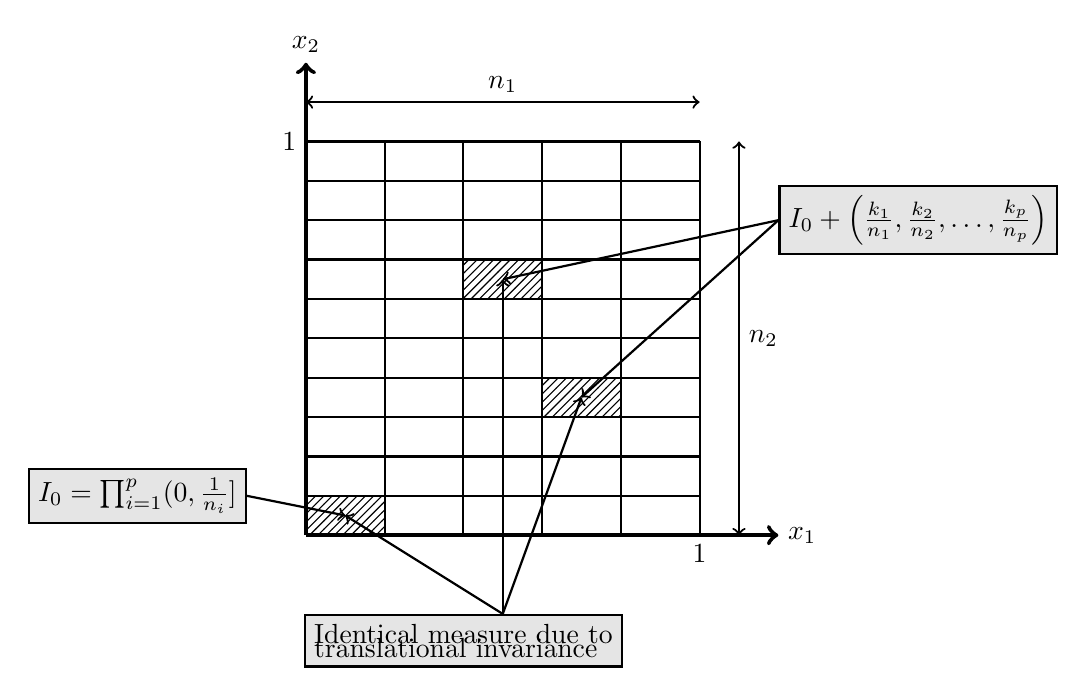
\begin{tikzpicture}[scale=5]
		\draw[ultra thick,->] (0,0) -- (1.2,0);
		\draw (1.2,0) node[anchor=west] {$x_1$};
		\draw[ultra thick, ->] (0,0) -- (0,1.2);
		\draw (0,1.2) node[anchor=south] {$x_2$};
		\draw[thick] (0,0) grid[xstep=0.2,ystep=0.1] (1,1);
		\fill[pattern = north east lines] (0,0) rectangle (0.2,0.1);
		\draw (1,0) node[anchor=north]{$1$};
		\draw (0,1) node[anchor=east] {$1$};
		\draw[thick, <->] (1.1,0) -- (1.1,1);
		\draw[thick, <->] (0,1.1) -- (1,1.1);
		\draw (0.5,1.1) node[anchor=south] {$n_1$};
		\draw (1.1,0.5) node[anchor=west] {$n_2$};
		\fill[pattern = north east lines] (0.4,0.6) rectangle ++(0.2,0.1);
		\filldraw (0.4,-0.2) node[anchor=north, align=left, draw, thick,fill=black!10] {Identical measure due to\\[-0.7em] translational invariance};
		\draw[thick, ->] (0.5,-0.2) -- (0.1,0.05);
		\draw[thick, ->] (0.5,-0.2) -- (0.5,0.65);
		\draw[thick, ->] (0.5,-0.2) -- (0.7,0.35);
		\filldraw (-0.15,0.1) node[anchor=east, draw, thick,fill=black!10] {$I_0=\prod_{i=1}^p (0,\frac{1}{n_i}]$};
		\draw[thick, ->] (-0.15,0.1) -- (0.1,0.05);
		\fill[pattern = north east lines] (0.6,0.3) rectangle ++ (0.2,0.1);
		\filldraw (1.2,0.8) node[anchor=west, draw, thick,fill=black!10] {$I_0+\left(\frac{k_1}{n_1}, \frac{k_2}{n_2},\dots, \frac{k_p}{n_p}\right)$};
		\draw[thick, ->] (1.2,0.8) -- (0.5,0.65);
		\draw[thick, ->] (1.2,0.8) -- (0.7,0.35);
	\end{tikzpicture}
\end{center}
Hence the Lebesgue Measure $\lambda$ and the new measure $\mu$ agree on all intervals of the form $\prod_{i=1}^p \left(0,\frac{1}{n_i}\right]$. The conclusion follows.
\end{proof}
\end{document}
